% Part: model-theory
% Chapter: interpolation
% Section: separation

\documentclass[../../../include/open-logic-section]{subfiles}

\begin{document}

\olfileid{mod}{int}{sep}

\olsection{\printtoken{P}{sentence}ల వేరుపరచడం}

అంతర్వేశ సిద్ధాంతపు నిరూపణకు వెళ్లేముందు కొంత పునాది పని కావాలి.
$!A$, $!B$లకు అంతర్వేశకం అంటే $!A \Entails !C$, $!C \Entails !B$
అయ్యే \tetoken{ఒక వాక్యం}{!!a{sentence}}~$!C$. విపర్యయ విధానం
ప్రకారం, రెండవది $\lnot !B \Entails \lnot !C$ అయినప్పుడు, అప్పుడు
మాత్రమే నిజం. ఈ ధర్మం గల \tetoken{ఒక వాక్యం}{!!^a{sentence}}~$!C$ అనేది
$!A$ను మరియు $\lnot !B$ను \emph{వేరుపరుస్తుంది} అంటారు. కాబట్టి
$!A$, $!B$లకు అంతర్వేశకాన్ని కనుగొనడమంటే $!A$, $\lnot !B$లను
వేరుపరిచే \tetoken{ఒక వాక్యాన్ని}{!!a{sentence}} కనుగొనడమే. తరచుగా
జరిగినట్లే, దీని సాధారణీకరణను---రెండు
\emph{\tetoken{వాక్యాల}{!!{sentence}s} సమితులను}
వేరుపరిచే ఒక వాక్యాన్ని---పరిశీలించడం ఉపయోగకరం.

\begin{defn}
$\Gamma$, $\Delta$ అనే వాక్యాల సమితులను $!C$ అనే వాక్యం
\emph{వేరుపరుస్తుంది} అంటే, అప్పుడు మాత్రమే $\Gamma \Entails !C$,
$\Delta \Entails \lnot !C$. అలాంటి \tetoken{వాక్యం}{!!{sentence}}
ఏదీ లేకపోతే $\Gamma$, $\Delta$లు \emph{వేరుపరచలేనివి}.
\end{defn}

$\Gamma$, $\Delta$, $!C$ల నమూనాల తరగతుల్లో ఏవి వేటిలో ఇమిడి ఉన్నాయో
కింద చూపించాం:
\begin{figure}[h]
  \centering
  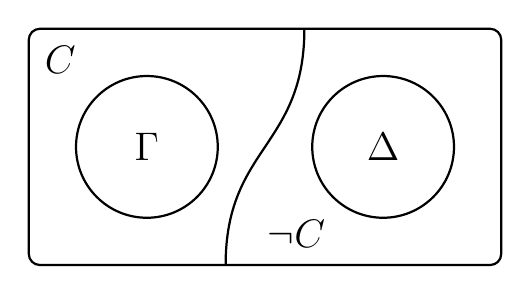
\begin{tikzpicture}[node distance=2cm, auto, thick]
    \draw [rounded corners] (0,0) -- (6,0) -- (6,3) -- (0,3) --  cycle;
    \draw (1.5,1.5) circle (0.9cm);
    \draw (4.5,1.5) circle (0.9cm);
    \path node at (1.5,1.5) {\Large $\Gamma$};
    \path node at (4.5,1.5) {\Large $\Delta$};
    \path node at (0.4,2.6) {\Large $\formula{C}$};
    \path node at (3.4,0.4) {\Large $\lnot \formula{C}$};
    \draw (2.5,0) .. controls (2.5,1.5) and (3.5,1.5) .. (3.5,3);
  \end{tikzpicture}
  \caption{$!C$ అనేది $\Gamma$, $\Delta$లను వేరుపరుస్తుంది}
  \ollabel{fig:sep}
\end{figure}

\begin{lem}\ollabel{lem:sep1}
$\Gamma$, $\Delta$ రెండింటిలోనూ వచ్చే ప్రతి
\tetoken{స్థిరసంకేతం}{!!{constant}},
\tetoken{ప్రమేయ సంకేతం}{!!{function}},
\tetoken{విధేయ సంకేతం}{!!{predicate}} ($\doteq$ తప్ప) కలిగిన భాష
$\Lang{L}_0$ అనుకుందాం; ప్రతి $n \ge 0$కు కొత్త
\tetoken{స్థిరసంకేతాలు}{!!{constant}s}~$\Obj c_n$ను చేర్చి
$\Lang{L}'_0$ను పొందామనుకుందాం. $\Lang{L}_0$లో $\Gamma$, $\Delta$లు
వేరుపరచలేనివైతే, $\Lang{L}'_0$లో కూడా అవి వేరుపరచలేనివే.
\end{lem}

\begin{proof}
పరోక్షంగా నిరూపిద్దాం: వైరుధ్యాన్ని పొందడానికి $\Lang{L}'_0$లో
$\Gamma$, $\Delta$లు వేరుపరచబడ్డాయని అనుకుందాం. అప్పుడు ఏదో
$!C \in \Lang{L}_0$కు $\Gamma \Entails \Subst{!C}{c}{x}$,
$\Delta \Entails \lnot \Subst{!C}{c}{x}$ (ఇక్కడ $c$ ఒక కొత్త
\tetoken{స్థిరసంకేతం}{!!{constant}}; $!C$లో ఇలాంటి కొత్త
\tetoken{స్థిరసంకేతాలు}{!!{constant}} ఒకటి కంటే ఎక్కువ ఉండే సందర్భం
కూడా ఇలాగే ఉంటుంది). సంహతత్వం వల్ల $\Gamma$లోని పరిమిత ఉపసమితి
$\Gamma_0$, $\Delta$లోని పరిమిత ఉపసమితి $\Delta_0$ ఉండి,
$\Gamma_0 \Entails \Subst{!C}{c}{x}$,
$\Delta_0 \Entails \lnot \Subst{!C}{c}{x}$ అవుతాయి. $\Gamma_0$లోని
అన్ని \tetoken{సూత్రాల}{!!{formula}s} సంయోగాన్ని $!G$గా,
$\Delta_0$లోని అన్ని \tetoken{సూత్రాల}{!!{formula}s} సంయోగాన్ని
$!H$గా ఉంచండి. అప్పుడు
\begin{align*}
  !G & \Entails \Subst{!C}{c}{x}, & !H  \Entails \lnot \Subst{!C}{c}{x}.
\end{align*}
మొదటిదాని నుంచి సార్వత్రీకరణ ద్వారా $!G \Entails
\lforall[x][!C]$ వస్తుంది. రెండవదాని నుంచి విపర్యయ విధానం ద్వారా
$\Subst{!C}{c}{x} \Entails \lnot !H$, అందువల్ల
$\lforall[x][!C] \Entails \lnot !H$ కూడా వస్తుంది.
\sourcecorrection{OLTEMODINT-001}{ఈ అనుగమనంలో ఆంగ్ల మూలం
$\lnot !H$ స్థానంలో నిర్వచించని $\lnot\delta$ను రాస్తుంది. వెంటనే
వచ్చే విపర్యయ అడుగు $!H \Entails \lnot\lforall[x][!C]$ కావాలంటే
ఇక్కడ సంయోగం $!H$నే ఉండాలి; దాన్ని పునరుద్ధరించాం.}
మళ్లీ విపర్యయ విధానం వల్ల $!H \Entails \lnot \lforall[x][!C]$.
ఏకదిశత ద్వారా
\begin{align*}
  \Gamma &\Entails \lforall[x][!C], &
  \Delta & \Entails \lnot \lforall[x][!C],
\end{align*}
కాబట్టి $\Lang{L}_0$లో $\lforall[x][!C]$ అనేది $\Gamma$, $\Delta$లను
వేరుపరుస్తుంది.
\end{proof}

\begin{lem}\ollabel{lem:sep2}
$\Gamma \cup \{ \lexists[x][!S] \}$, $\Delta$లు వేరుపరచలేనివని,
$c$ అనేది $\Gamma$, $\Delta$, $!S$లలో రాని కొత్త
\tetoken{స్థిరసంకేతం}{!!{constant}} అని అనుకుందాం. అప్పుడు
$\Gamma \cup \{ \lexists[x][!S], \Subst{!S}{c}{x} \}$, $\Delta$లు
కూడా వేరుపరచలేనివే.
\end{lem}

\begin{proof}
$!C$ అనేది $\Gamma \cup \{\lexists[x][!S], \Subst{!S}{c}{x}\}$ను,
$\Delta$ను వేరుపరుస్తుందని, అదే సమయంలో
$\Gamma \cup \{\lexists[x][!S] \}$, $\Delta$లు వేరుపరచలేనివని
వైరుధ్యం కోసం అనుకుందాం.
\sourcecorrection{OLTEMODINT-002}{ఈ పరికల్పనను మళ్లీ రాసిన చోట
ఆంగ్ల మూలం ఒక్కసారి $\lexists[x]{!S}$ అని వాడి, ఈ ఘనీభూతంలోని
మిగతా ప్రతి ప్రయోగానికి భిన్నంగా పరిమాణీకృత సూత్రాన్ని ఐచ్ఛిక
ఆర్గ్యుమెంటు వెలుపల ఉంచుతుంది. ఉద్దేశించిన $\lexists[x][!S]$ను
పునరుద్ధరించాం.}
రెండు సందర్భాలను వేరు చేద్దాం:
\begin{enumerate}
\item $!C$లో $c$ రాదు: ఈ సందర్భంలో $\Gamma \cup
  \{\lexists[x][!S], \lnot!C \}$ సంతృప్తిపరచదగినది (లేకపోతే $!C$ అనేది
  $\Gamma \cup \{\lexists[x][!S] \}$ను, $\Delta$ను వేరుపరుస్తుంది).
  $\Subst{!S}{c}{x}$ను చేర్చినా అది సంతృప్తిపరచదగినదిగానే ఉంటుంది;
  కనుక చివరికి $!C$ అనేది $\Gamma \cup \{ \lexists[x][!S],
  \Subst{!S}{c}{x} \}$ను, $\Delta$ను వేరుపరచదు.
\item $!C$లో $c$ వస్తుంది; అందువల్ల $!C$కు
  $\Subst{!C}{c}{x}$ రూపం ఉంటుంది. అప్పుడు
  \[
  \Gamma \cup \{ \lexists[x][!S], \Subst{!S}{c}{x}\} \Entails \Subst{!C}{c}{x},
  \]
  నిగమన సిద్ధాంతం, సార్వత్రీకరణ ద్వారా
  $\Gamma, \lexists[x][!S] \Entails \lforall[x][(!S \lif !C)]$;
  చివరికి $\Gamma \cup \{ \lexists[x][!S] \} \Entails
  \lexists[x][!C]$. మరోవైపు,
  $\Delta \Entails \lnot \Subst{!C}{c}{x}$; అందువల్ల సార్వత్రీకరణ
  ద్వారా $\Delta \Entails \lnot \lexists[x][!C]$. కాబట్టి
  $\Gamma \cup \{\lexists[x][!S] \}$, $\Delta$లు వేరుపరచదగినవి;
  ఇది వైరుధ్యం.
\end{enumerate}
\end{proof}

\end{document}
